\section{Statistical Analysis}
\subsection{Engagement}
A Q-Q visual test revealed that the number of times participants recorded is not normally distributed~\cite{das2016brief}. Since the samples are not independent, we used the Friedman test to determine statistical significance~\cite{sheldon1996use}. We found that participants recorded more with \visowel{} practice than with audio-only (p=0.0339). Because the visualization in \visowel{} depended on speaker, we tested for a difference between participants who practiced with a female voice (N=4) versus a male voice and did not find a statistically significant difference (p=1).
\subsection{NASA-TLX}
In order to determine the suitability of performing an ANOVA on average NASA scores~\cite{st1989analysis}, we used visual Q-Q graphs to see how much our distribution varied from a normal distribution. We compared the visual results with a Shapiro-Wilk numerical test and determined that the data could be considered to be pulled from a normal distribution (Figure \ref{fig:nasascore}). We performed a two-factor ANOVA without Replication on the average NASA TLX scores collected after the baseline check, audio-only, and \visowel{} practices (p=0.008). We excluded the baseline scores in a second ANOVA and found that there was no statistical difference between the load of \visowel{} and audio-only practices (p=0.102), which is expected since the baseline condition does not require thinking about pronunciation.
\subsection{System Usability Scores}
A test for normalcy in the distributions showed that the \visowel{} scores were close to a normal distribution, but the audio-only was not. As a result, we used the Friedman test to determine if the difference in usability between the tools was statistically significant. There was no statistical difference in usability (p=0.480).

\section{Motivation}
To better understand learning goals, we had participants complete a motivation survey, modeled after the mini-AMTB by Tennant and Gardner~\cite{tennant2004computerized}. The survey gauges the motivation behind learning Spanish using five point Likert scales. 

The overall motivation of a participant as defined by Tennant and Gardner is:
\begin{align*}
    MOTIV = MI + D + AL\label{eq:motiv}
\end{align*}
% \[MOTIV = MI + D + AL\]\label{eq:motiv}

where MI is the numerical response to the motivation question, D is the response to the desire question, and AL is the attitude toward learning the target language (see Appendix \ref{app:motiv} for a list of questions). To return to a 5-pt Likert scale, we divide the result by 3.
\subsection{Questions}
\label{app:motiv}
\paragraph{Integrative Orientation (IO)} If I were to rate my feelings about learning Spanish in order to interact with Hispanic or Latino speakers, I would have to say they are, "weak ... strong" 
\paragraph{Attitude toward Hispanic or Latino Americans (AFA)} My attitude toward Hispanic or Latino speakers is, "unfavorable ... favorable" 
\paragraph{Interest in Foreign Languages (IFL)} My interest in languages other than Spanish and English is, "very low ... very high"
\paragraph{Desire to learn Spanish (D)} My desire to learn Spanish is: "weak ... strong"
\paragraph{Attitude toward learning Spanish (AL)} My attitude toward learning Spanish is: "unfavorable ... favorable"
\paragraph{Instrumental Orientation (IO)} If I were to rate my feelings about learning Spanish for practical purposes such as to improve my occupational opportunities, I would have to say they are "weak ... strong"
\paragraph{Motivational Intensity (MI)} I would characterize how hard I work at learning Spanish as "very little ... very much"
\section{Results}
\begin{table}[]
    \begin{tabular}{l|ccc||c}
    ID & D & \makecell{MI} & \makecell{ALSpa} & Average MOTIV \\
    \hline
    P2             & 4                           & 3                           & 5                                        & 4.0           \\
    P3             & 5                           & 3                           & 5                                        & 4.0           \\
    P4             & 5                           & 3                           & 5                                        & 3.7           \\
    P5             & 5                           & 5                           & 5                                        & 5.0           \\
    P6             & 4                           & 3                           & 5                                        & 3.7           \\
    P7             & 4                           & 4                           & 5                                        & 4.0           \\
    P8             & 4                           & 2                           & 5                                        & 3.3           \\
    P9             & 4                           & 2                           & 5                                        & 3.3          
    \end{tabular}
    \caption{Responses to the motivation questionnaire, where average motivation is calculated as
    ( Desire + Motivational Intensity + Attitude toward Learning Spanish ) / 3}
    \label{tab:motiv}
\end{table}

The participants all had a greater than 3 average motivation to learn Spanish (Table \ref{tab:motiv}). The motivation to engage with Spanish practice is reinforced by the thoughtful comments participants made during practice (Sections \ref{sec:AudFeed} and \ref{sec:VisFeed} ).

\section{Exit Interview Questions}
Each question was asked for both practices.
\begin{itemize}
    \item How did you like the feedback?
    \item How was the feedback useful? 
    \begin{itemize}
        \item What feedback could you act on?
    \end{itemize}
    \item How trustworthy was the feedback?
    \item What did you find confusing or distracting?
\end{itemize}

\section{Design Decisions}
\label{app:design}
\subsection{Color Palettes}
\label{app:palette}
\begin{figure}[h]
    \centering
    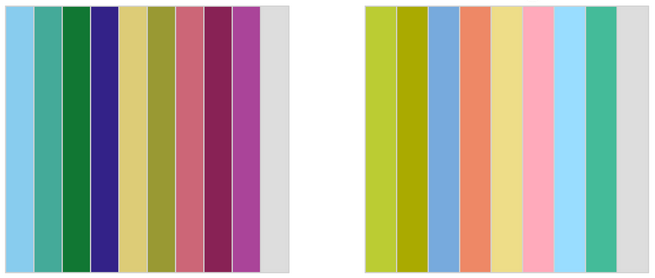
\includegraphics[width=0.5\textwidth]{pictures/colorblindPalette.png}
    \caption{Two colorblind friendly palettes. From left to right: tol\_muted and tol\_light.}
    \label{fig:colorblind}
\end{figure}
We considered colorblind friendly colors for differentiating the words and speakers, green and purple for Spanish, and blue and red for the learner (Figure \ref{fig:visowelPrac}). 

% Since we wanted participants to interact with the Spanish lines on the chart, we initially plotted both Spanish recordings in orange. Participants expressed confusion during interaction, so we gave the words different colors. 

\subsection{Layout}
\label{app:layout}
\begin{figure*}[t]
    \centering
    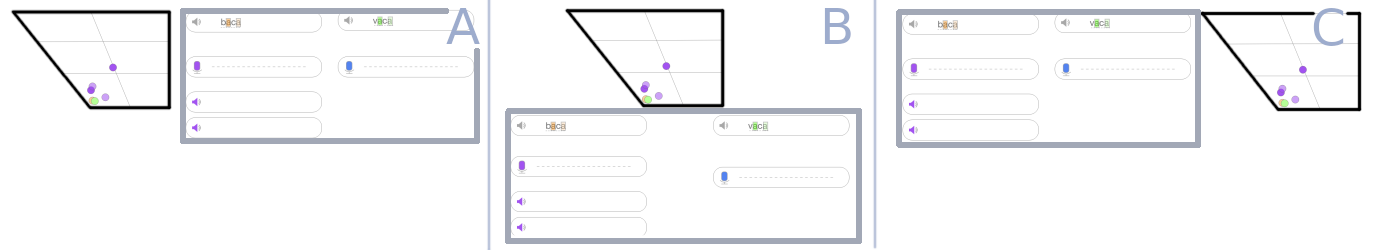
\includegraphics[width=\linewidth]{pictures/layoutsOutline.png}
    \caption{Three potential layouts for \visowel{} practice. The vowel chart is outlined in black and the recording buttons and recordings are outlined in grey. Audio-only practice is just the grey portion.}
    \label{fig:layouts}
\end{figure*}
We evaluated three potential layouts for the minimal pair recording buttons and \visowel{} (Figure \ref{fig:layouts}). The layouts represented the potential orderings that were possible given the chart and buttons. We ended with a horizontal alignment of the buttons with the chart because the vowel chart has a straight side which makes the best use of the available space. 

\section{Tutorial}
\label{app:tutorial}
\begin{figure}[h]
    \centering
    \begin{subfigure}{\linewidth}
        \centering
        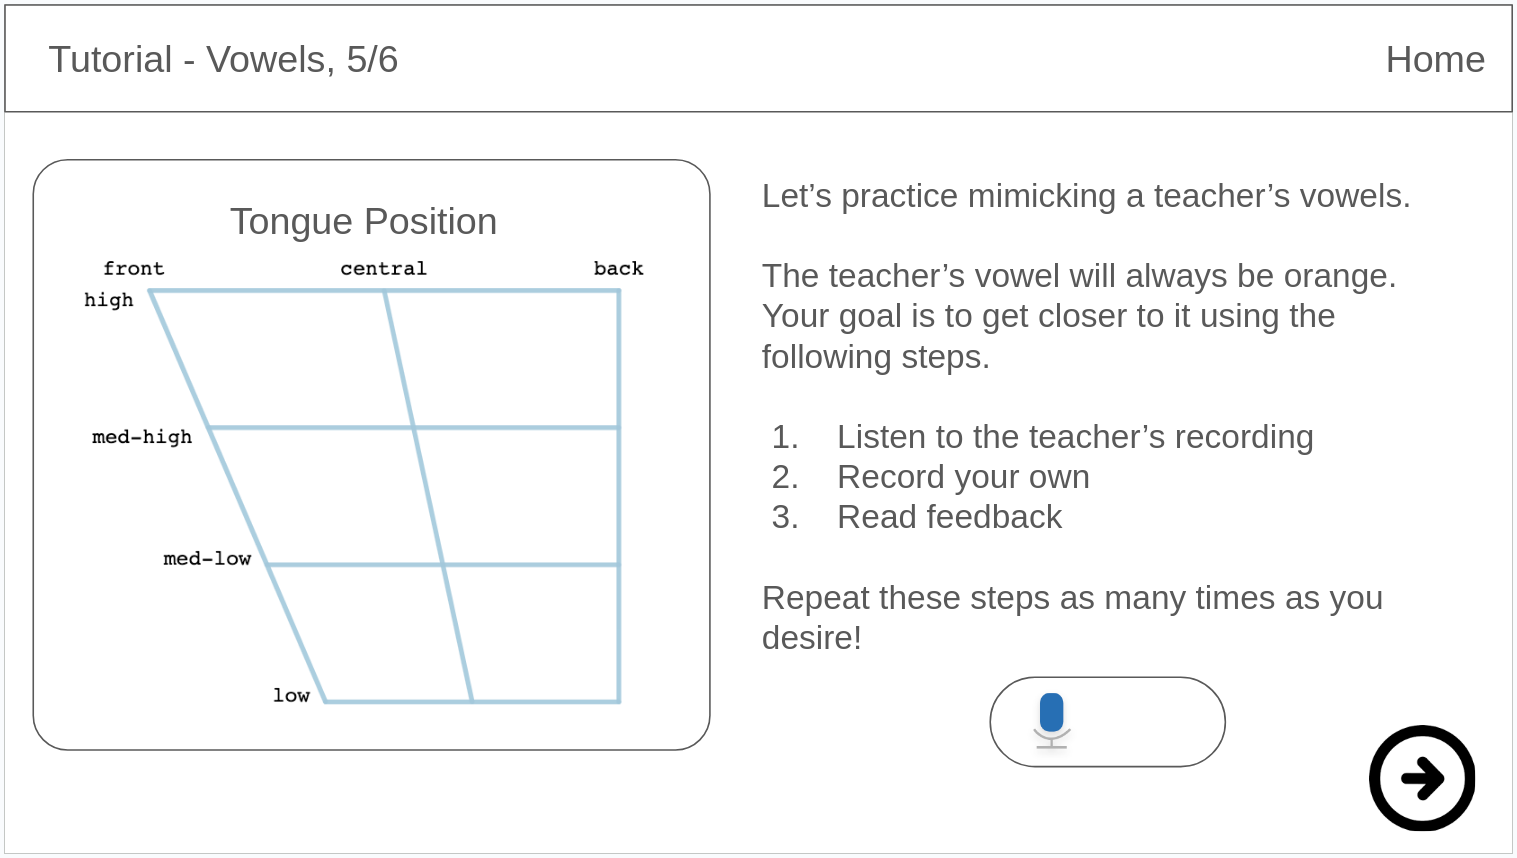
\includegraphics[width=0.9\linewidth]{pictures/tutorial/tut5paper.png}
        \caption{Paper prototype of tutorial page 5. The user is introduced to the idea of the Spanish speaker's line by recording the Spanish word.}
        \label{fig:5tutPaper}
    \end{subfigure}
 
    \begin{subfigure}{\linewidth}
        \centering
        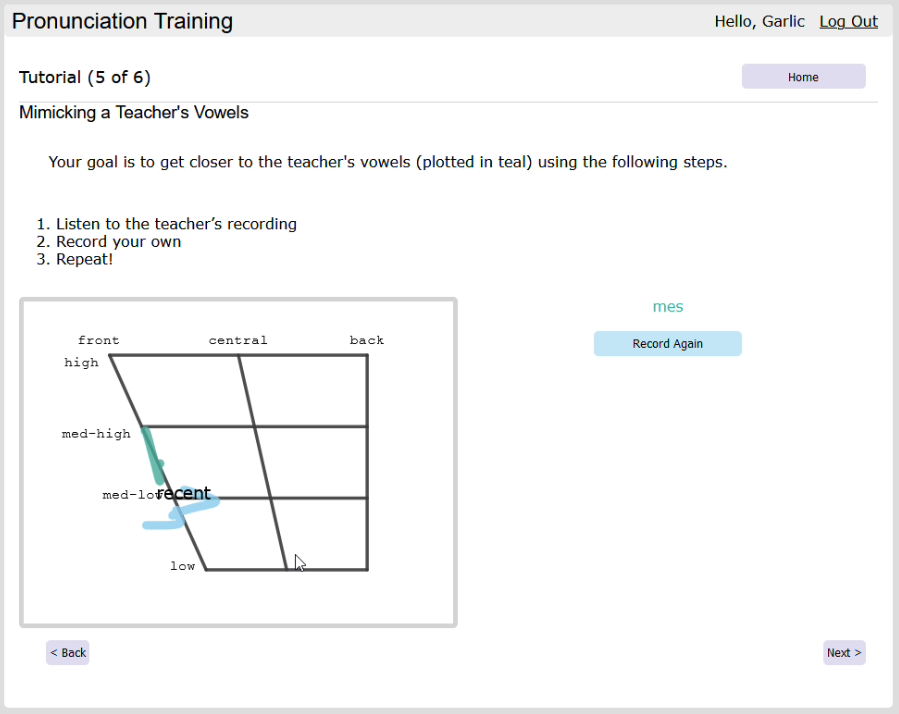
\includegraphics[width=0.825\linewidth]{pictures/tutorial/tut5.png}
        \caption{Final interface for the tutorial's fifth page. The user can click on the Spanish speaker's line to hear the word and record their own version of it.}
        \label{fig:5tut}
    \end{subfigure}
    
    \caption{Three pages representative pages taken from the tutorial. The images on the right are the initial paper prototype and the ones on the left are the final rendition of the corresponding pages.}
    \label{fig:tutorialPages}
\end{figure}
The tutorial begins with face-cutaways that show the position of the tongue during the production of four different vowels in extreme positions (two front vowels, high and low, and two back vowels, high and low. See Figure \ref{fig:1tutPaper}). The second page we introduce the vowel chart alongside a face-cutaway to show correlation between the position of the tongue and the points on the chart. The third and fourth steps break down the horizontal and vertical axes by bringing attention to the position of the tongue to a user and letting them record English words that differ in the respective axis. After allowing users to interact with English words, we presented them with the idea of getting close to a Spanish recording. The final step was a review of the tongue's mapping to the vowel chart.  
\begin{figure}[h]
    \centering
    \begin{subfigure}{\linewidth}
        \centering
        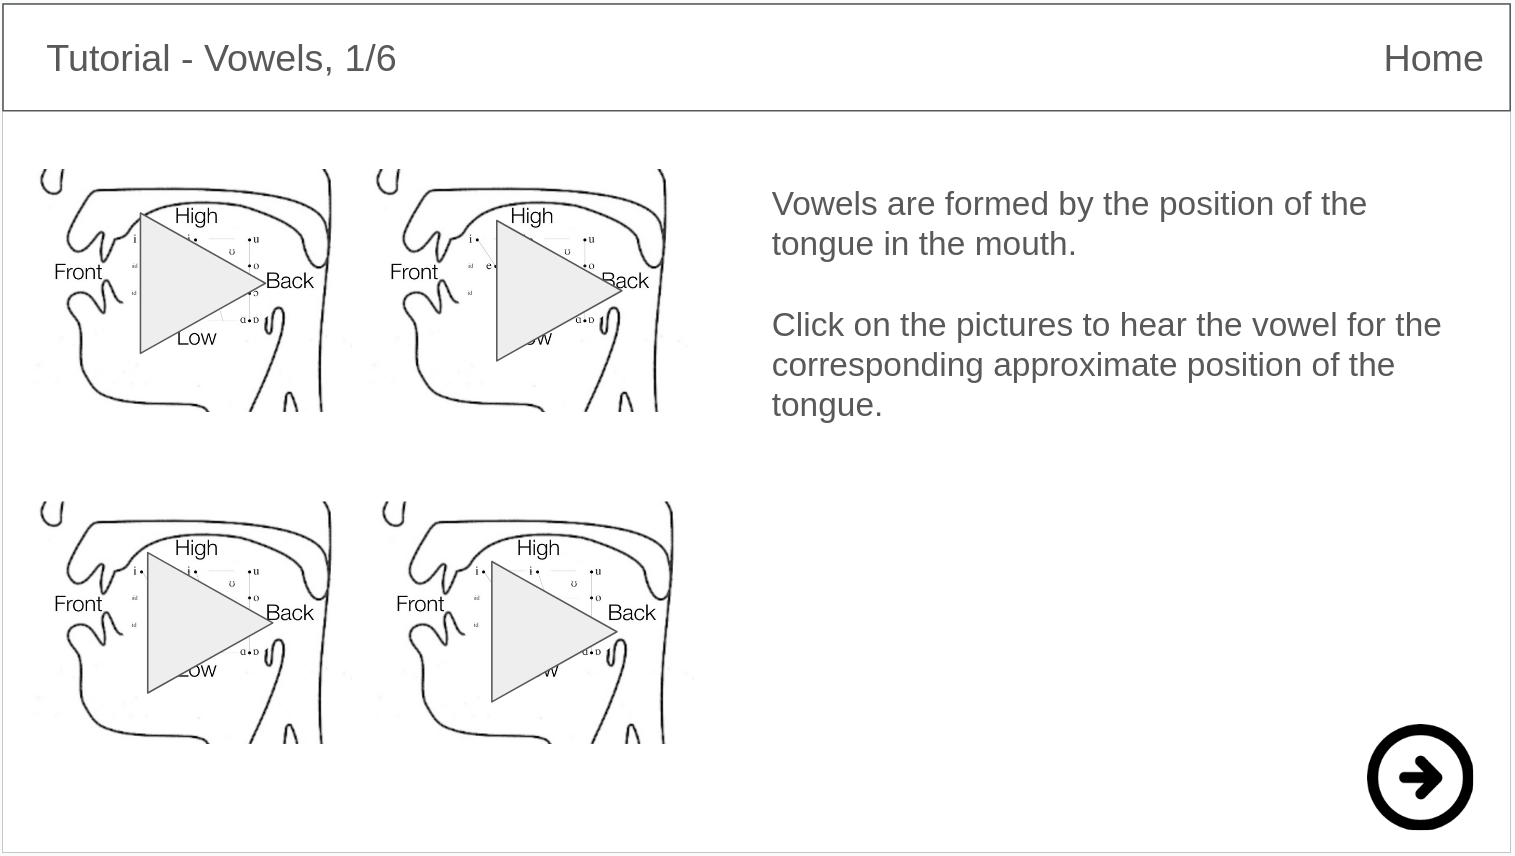
\includegraphics[width=0.9\linewidth]{pictures/tutorial/tut1paper.png}
        \caption{The paper prototype of the first page of the tutorial. A grid of four face cutaways is on the left. Triangles on each of the pictures indicated that they were short videos.}
        \label{fig:1tutPaper}
    \end{subfigure}%

    \begin{subfigure}{\linewidth}
        \centering
        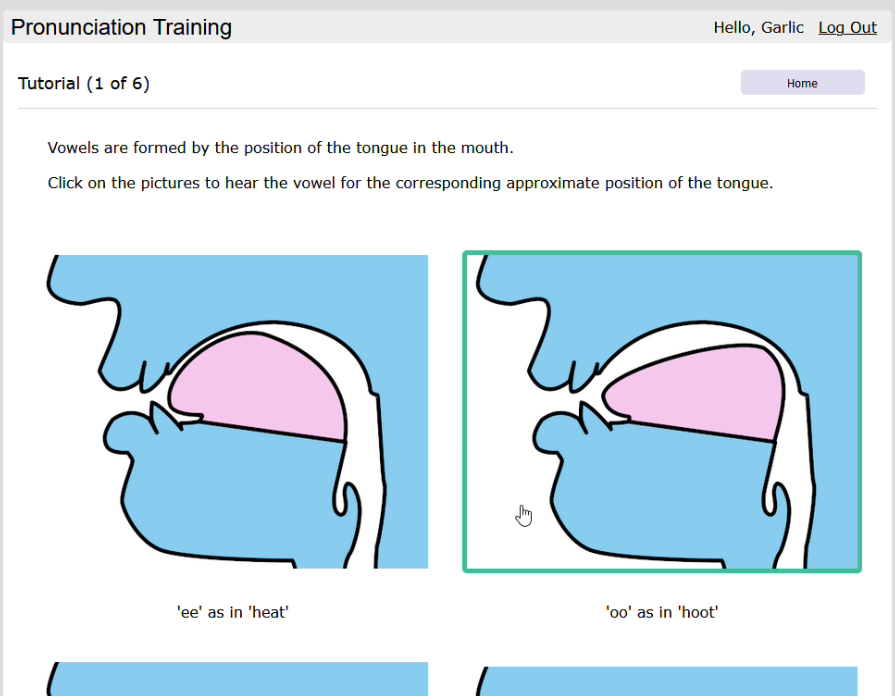
\includegraphics[width=0.8\linewidth]{pictures/tutorial/tut1.png}
        \caption{Final interface for the tutorial's first page. The face cutaways are static due technical limitations. Hovering over a picture lines it with green indicating that a user can interact with it.}
        \label{fig:1tut}
    \end{subfigure}
    \label{fig:pg1}
    \caption{Design cycle of page 1}
\end{figure}
Based on pretests, we modified the tutorial to include the same four vowels to cement the association from the first step (Figure \ref{fig:2tut}). We created an interactive prototype and ran another pretest. We learned that people were unaware that the face cutaways on the first page were interactive. When clicked, they played the associated vowel. To bring attention to the interaction, we show an outline when the mouse hovers over any of the pictures (Figure \ref{fig:1tut}). Originally, all the vowels on the second page were the same color. Based on feedback, we colored the tongues to match the colors of the vowels on the chart to create a visual association. An overall modification we made based on pretest information was to put the instructions above the vowel chart to encourage users to read the instructions before plowing ahead. We also pared down the instructions to be more concise.

\section{Vowel Boundary Algorithms}
\label{app:algo}
We outline brief descriptions of the algorithms we tested for vowel boundary extraction and why we did not use them. 

We started using a DTW algorithm~\cite{bellman1959dtw}, which maps similar points between two audio samples regardless of speed. There were two flaws with DTW. First, if an English speaker didn't pronounce the consonants like the Spanish reference, then the mapping would include multiple points near the beginning of the vowel, potentially throwing off the beginning and ending boundaries for the vowel (Figure \ref{fig:DTW}). Second, even when DTW was accurate, the window size could not be made small enough (<10ms) to exclude enough of the consonant in the extraction. 

Next, we tested extracting timestamps by using pocketSphinx (PS)~\cite{huggins2006pocketsphinx}. PS is a speaker-independent continuous speech-recognition algorithm begun by Huggins-Daines et. al. It takes in an audio file and returns the phones and silences with associated timestamps detected in the file. The timestamps had a similar degree of inaccuracy as DTW.

We decided to test Praat's vowel extractor suitability for extraction using the parselmouth library, a python interface for Praat~\cite{jadoul2018introducing}. The original Praat script written by Hugo Quené only extracts a portion of the vowel so we modified the script to output the timestamps for the whole vowel~\cite{hugoQuenePraat}. The boundaries using this method were also inaccurate. 

\section{Timing Considerations}
% Timing considerations
We wanted to keep the timing between recording and visualization low. Some parts of the server side code have a set amount of time: speech recognition, vowel boundary and formant extraction. While the algorithm ran these processes, we displayed "Processing" on the record button and disabled interaction with it. For the formants to be displayed on the chart, they must be transformed from the frequency to svg domain. Initially, we transformed each pair of formants, $f_1$ and $f_2$, one by one. We optimized the process by transforming formants in a batch. 